%! TEX root = ../root/raiz.tex
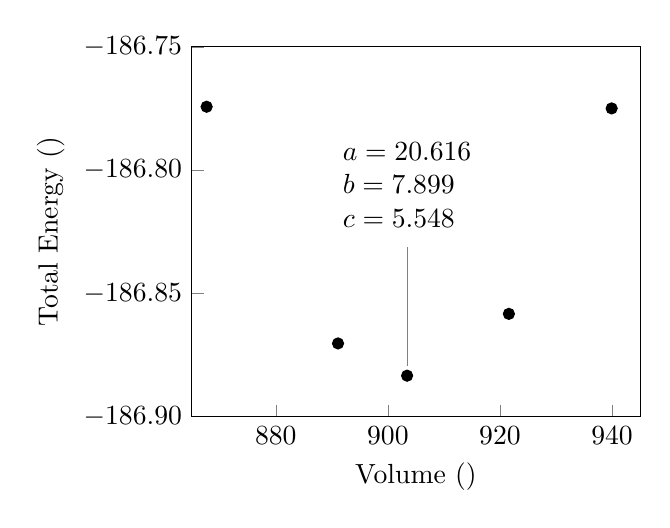
\begin{tikzpicture}
    \begin{axis}
        [
            width=.6\linewidth,
            legend pos={outer north east},
            legend style={draw=none},
            legend cell align=left,
            tick align=inside,
            tick pos=left,
            minor tick num=0,
            xlabel={Volume (\si{\cubic\angstrom})},
            xmin=865,xmax=945,
            xticklabel style={
                /pgf/number format/.cd,
                1000 sep={}
            },
            ylabel={Total Energy (\si{\electronvolt})},
            ymin=-186.9,ymax=-186.75,
            yticklabel style={
                /pgf/number format/.cd,
                1000 sep={},
                fixed,
                fixed zerofill,
                precision=2,
                /tikz/.cd
            },
        ]
        \addplot [black, only marks, mark=*] table {
        867.6555578005446 -186.77428847
        891.1015000000002 -186.87035702
        903.43            -186.88344643
        921.5904149441228 -186.85835686
        939.9300732358251 -186.77495984
        }
        node [pin={[pin distance=10ex]90:\begin{tabular}{l}$a=\SI{20.616}{\angstrom}$\\$b=\SI{7.899}{\angstrom}$\\$c=\SI{5.548}{\angstrom}$\\\end{tabular}}] at (903.43, -186.88344643) {};
    \end{axis}
\end{tikzpicture}
